\section{Wstęp}
    Celem poniższej pracy jest skonstruowanie autonomicznego pojazdu, którego zadaniem będzie zbudowanie wirtualnej mapy terenu oraz samodzielne poruszanie się po nieznanym obszarze.
    Jednym z założeń projektu jest umożliwienie użytkownikowi kontroli nad pojazdem za pomocą dedykowanej aplikacji komputerowej.
    Dodatkowo, powyższa aplikacja będzie wyświetlać budowaną mapę w czasie rzeczywistym.
    Po wskazaniu punktu docelowego, zostanie zaproponowana optymalna trasa, po której pojazd będzie się poruszał.


    \subsection{Środowisko sprzętowe}
    \label{subsec:hardware}
        Współczesne pojazdy autonomiczne wyposażone są w jednostki obliczeniowe, które swoją konstrukcją przypominają pełnoprawne komputery z systemem operacyjnym.
        Ten projekt ma być modelem,  przedstawiającym działanie pojazdu autonomicznego, dlatego wykorzystanie pełnoprawnego komputera jest zbędne.

        \subsubsection{Mikrokontroler}
            Poniżej przedstawiono kilka najbardziej popularnym platform sprzętowych, które mogą stanowić bazę dla pojazdu.
            \begin{enumerate}
                \item Raspberry Pi -- komputer z systemem operacyjnym Linux, umożliwiający bezpośredni dostęp do modułów zewnętrznych z pomocą GPIO.
                Jest to najbardziej popularna platforma dla projektów DIY.
                Układ pozwala na niesamowitą elastyczność w pracy, między innymi na podłączenie się do układu za pośrednictwem SSH oraz pracę w języku Python.
                Jednak ze względu na swoją popularność, jest bardzo drogi i mało dostępny.
                Natomiast, jednym z założeń projektu jest działanie w czasie rzeczywistym, co przy wykorzystaniu systemu operacyjnego jest niemożliwe.
                \item Arduino -- najpopularniejsza platforma, której głównymi zaletami są: prostota framework'u oraz mnogość bibliotek dla każdego układu.
                Niestety, płytki te oparte są o 8-bitowe mikrokontrolery z rodziny AVR, co odbija się na ich prędkościach  (max 20MHz).
                Sam framework wykorzystywany jest na wielu różnych praformach, przez co w dłuższej perspektywie staje się nieintuicyjny.
                \item STM32 -- układy projektowane przez firmę STMicroelectronics. Są znacznie szybsze i posiadają więcej pamięci od Arduino.
                Jednak ze względu na potrzebę wykorzystania biblioteki HAL, programowanie jest znacznie trudniejsze w porównaniu do innych układów.
                \item ESP32 -- 32-bitowy dwurdzeniowy procesor z wbudowanym modułem WiFi i Bluetooth.
                Jeden z najszybszych mikrokontrolerów dostępnych na rynku. Jest bardzo popularny w projektach IoT (wytłumaczyć).
                Natywnie pracuje w systemie czasu rzeczywistego - FreeRTOS. Dzięki temu ma potencjał na bycie idealnym kandydatem do tego projektu.
                Jednak znikoma dokumentacja produktu sprawia, że praca z nim jest uciążliwa, przez co opracowanie optymalnego kodu jest znacząco utrudnione.
                \item Raspberry Pi Pico -- mikrokontroler od firmy Raspberry Pi, oparty na rdzeniach Cortex - tak samo jak STM32.
                Producent udostępnił wyjątkowo przystępny zestaw narzędzi programistycznych oraz przykładów użycia.
                Kolejną z zalet jest dobra dokumentacja tego procesora, która jest stale rozwijana.
                W 2022 roku, pojawiła się druga iteracja tej płytki Raspberry Pi Pico~W ze zintegrowanym modułem WiFi.
            \end{enumerate}
            Projekt jest możliwy do zrealizowania na wszystkich wymienionych powyżej platformach.
            Jednak ze względu na swoją przystępność, Raspberry Pi Pico jest najbardziej optymalnym wyborem.
            \begin{figure}[!ht]
                \centering
                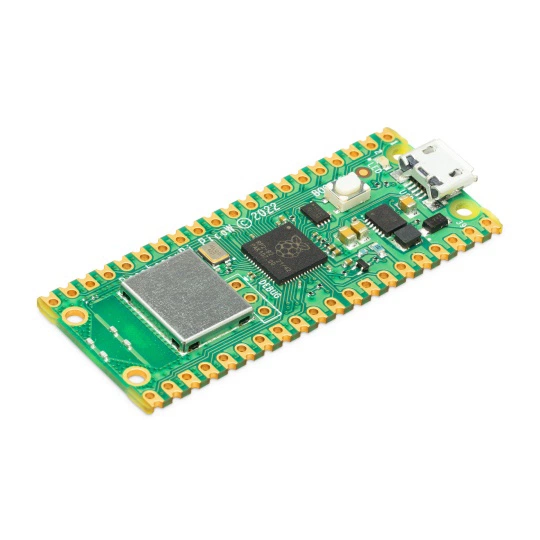
\includegraphics[width = 0.3\textwidth]{raspberry_pico.png}
                \caption{Raspberry Pi Pico}
                Źródło: \href{https://botland.com.pl/moduly-i-zestawy-do-raspberry-pi-pico/21574-raspberry-pi-pico-w-rp2040-arm-cortex-m0-cyw43439-wifi-5056561803173.html}{botland.com}

                % Źródło: https://botland.com.pl/silniki-dc-z-przekladnia-i-enkoderami/6287-silnik-z-przekladnia-sj01-120-1-6v-160rpm-enkoder-6959420910205.html
                % Źródło: https://botland.com.pl/serwa-typu-micro/20435-serwo-mg-90s-micro-180-stopni-metalowa-przekladnia-5904422380915.html
                \label{fig:raspberry_pico}
            \end{figure}

        \subsubsection{Sterowanie}
        \label{sec:engines}
            Podstawowym zadaniem pojazdów mechanicznych jest poruszanie się.
            Dlatego niezwykle istotne było wybranie odpowiedniego silnika napędowego.
            Na rynku konsumenckim istnieje jest wiele ich wariantów.
            Poniżej opisano możliwe rozwiązania oraz skrótowo omówiono ich wady i zalety:
            \begin{enumerate}
                \item Silniki krokowe -- niegdyś bardzo duże i drogie silniki, wymagające dodatkowych układów sterujących.
                Dziś jednak istnieją mniejsze, niskonapięciowe rozwiązania, które mogą być kontrolowaneZ bezpośrednio przez mikroprocesor.
                Niestety złożone sterowanie oraz niewielka prędkość maksymalna $v_{max} \approx 1 \frac{\text{obr.}}{s}$ sprawiają, że wykorzystanie ich w tym projekcie byłoby nieoptymalne.
                \item Serwomechanizmy $360^\circ$ -- silniki wraz z kontrolerem oraz przekładniami.
                Wbudowany układ pozwala na regulację prędkości z wysoką dokładnością.
                Nie ma jednak możliwości sprawdzenia, czy dwa moduły pracują z tą samą mocą.
                Może to prowadzić do wielu niepożądanych zachowań, jak na przykład trudności poruszaniem się w linii prostej.
                \item Serwomechanizmy $180^\circ$ -- ta odmiana pozwala na precyzyjne ustawienie pożądanego kąta.
                Układy te nie nadają się do napędzania pojazdów, gdyż ich zakres ruchu jest ograniczony do 180(stopni). Jednak, świetnie odnajdują się w sytuacjach, w których precyzja jest kluczowa.
                \item Silniki BLDC -- pozwalają osiągnąć bardzo wysokie prędkości.
                Niestety łączy się to z niemałą ceną.
                Dodatkowo każdy silnik wymaga wyspecjalizowanych układu sterującego.
                \item Silniki DC -- urządzenia elektromechaniczne przetwarzające moc prądu stałego na energię mechaniczną.
                Pozwalają na regulację prędkości za pomocą PWM.
                Dodatkowo w sprzedaży dostępne są układy wyposazone w enkodery, pozwalające obliczyć średnią prędkość silnika, a w konsekwencji wyznaczyć różnicę w pracy między nimi.
            \end{enumerate}
            Układ napędowy został oparty na silnikach DC z zamontowanymi enkoderami.
            Dzięki czemu możliwy jest odczyt prędkości pojazdu, który pozwala na wprowadzanie korekty szybkości.
            Natomiast, do układu kierowniczego, najlepiej nada się serwomechanizm $180^\circ$, ze względu na możliwość precyzyjnego ustawienia kąta. Oba wybrane układy przedstawiono poniżej \ref{fig:engines}.
            \begin{figure}[!ht]
                \centering
                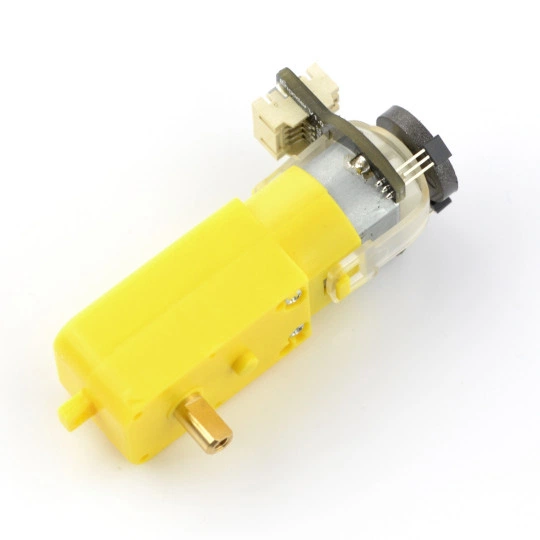
\includegraphics[width = 0.3\textwidth]{silnik_z_enkoder.png}
                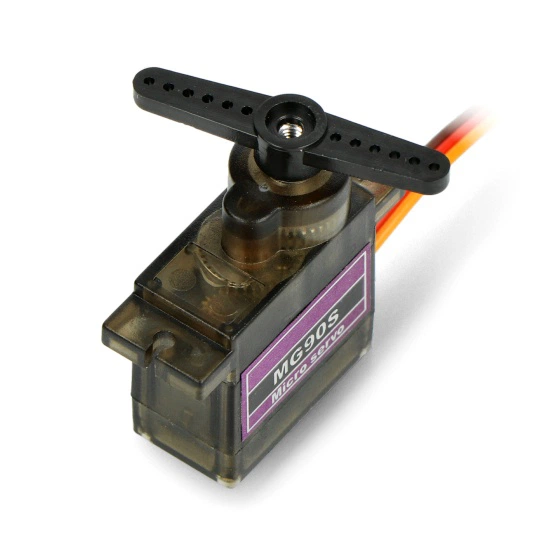
\includegraphics[width = 0.3\textwidth]{serwo_180.png}

                \caption{Silnik DC z enkoderem oraz serwomechanizmy $180^\circ$.}
                \footnotesize{Źródło: \href{https://botland.com.pl/}{botland.com}}
                % Źródło: https://botland.com.pl/silniki-dc-z-przekladnia-i-enkoderami/6287-silnik-z-przekladnia-sj01-120-1-6v-160rpm-enkoder-6959420910205.html
                % Źródło: https://botland.com.pl/serwa-typu-micro/20435-serwo-mg-90s-micro-180-stopni-metalowa-przekladnia-5904422380915.html
                \label{fig:engines}
            \end{figure}

        \subsubsection{Pomiar odległości}
            Praca pojazdów autonomicznych nie ogranicza się wyłącznie do sterowania silnikami.
            Urządzenia tego typu muszą być świadome swojego otoczenia.
            Zastosowanie odpowiednich czujników umożliwiających pomiar odległości jest niezbędne w celu zapewnienia bezkolizyjnej jazdy.
            % Autonomia pojazdu nie ogranicza się wyłącznie do sterowania silnikami.
            % Pojazd tego typu musi być świadomy swojego otoczenia.
            % Taką funkcjonalność mogą zapewnić czujniki służące do pomiaru odległości.
            % Ta funkcja wymaga wykorzystania czujników pozwalających na pomiar odległości.
            Poniżej przedstawiono listę różnych rodzajów czujników:
            \begin{enumerate}
                \item Czujniki ultradźwiękowe -- najpopularniejsze układy wykorzystywane do pomiaru odległości.
                Niewątpliwą zaletą jest prostota działania, jednak okupiona jest ona długim czasem wykonywania pomiarów.
                Co więcej uzyskane wartości obarczone są niepewnością, skutkującą znacznym odchyleniem od średniej.
                % Co więcej ich pomiary bywają niestabilne.
                \item Czujniki Time of Flight (ToF) -- wyspecjalizowane moduły o wysokiej dokładności, pozwalają na pomiary na znacznych odległościach.
                Zazwyczaj wymagają odpowiednich bibliotek dostarczonych przez producentów, co stanowi zarówno wadę jak i zaletę.
                Takie czujniki mogą pracować bardzo szybko jednak złożona, uniwersalna biblioteka spowalnia cały proces.
                \item Układy obiciowe IR -- obwody składające się z dwóch diod: emitera i odbiornika.
                Cechują się niewielkim zakresem pomiarowym (od $2cm$ do $20cm$) i znikomą dokładnością (pomiar zależy od koloru obiektu) oraz zauważalną strefą martwą.
                \item Lidar -- wyspecjalizowane układy, umożliwiające bardzo precyzyjny określenie odległości w pełnym zakresie $360^\circ$.
                Sprawia to, że jest jedną z najlepszych dostępnych opcji, jednak ceny takich układów są zaporowe.
                \item Radar -- niezwykle dokładne i kosztowne układy pomiarowe, pozwalające na nieporównywalną precyzję.
                Niestety ich rozmiar wymagany do tego projektu jest trudno dostępny na rynku konsumenckim.
                Co gorsza obowiązkowym staje się zastosowanie specjalnych procesorów sygnałowych, pozwalających na bieżąco przetwarzać dane z radarów.
            \end{enumerate}
            % Z wyżej przedstawionej listy, układami które sprawdzą się najlepiej w tym projekcie są czujniki typu ToF, zamontowane z przodu pojazdu.
            Z wyżej przedstawionej listy, w tym projekcie najlepiej sprawdzą się moduły ToF, zamontowane z przodu pojazdu.
            Dodatkowo ze względów bezpieczeństwa, z tyłu umieszczone zostały czujniki IR.
            Natomiast, nie są one wykorzystywane w charakterze urządzenia pomiarowego, tylko jako czujniki zbliżeniowe, umożliwiające wykrycie przeszkody i reakcję na niebezpieczeństwo.

    \subsection{Środowisko programistyczne}
        Następnym kluczowym wyborem jest środowisko programistyczne, w którym zostanie zbudowany projekt.
        % W ostatnich latach użytkownicy dostali bardzo dużo wolności w tej kwestii.
        W ostatnich latach powstało wiele narzędzi, pozwalających na dostosowanie całości do własnych potrzeb.
        Najpopularniejszymi narzędziami do programowania mikrokontrolerów są:
        \begin{enumerate}
            \item Eclipse -- kiedyś bardzo popularny program, posiadający olbrzymi zbiór rozszerzeń.
            Rozprowadzany na otwartej licencji, dlatego stanowi doskonałą bazę dla wielu bardziej zaawansowanych projektów.
            \item STM32 Cube -- środowisko przeznaczone głównie do pracy z modułami STM32, oparte na wyżej wymienionym Eclipse.
            \item Microchip Studio -- zbiór narzędzi wyspecjalizowanych do pracy z mikrokontrolerami z rodziny AVR od firmy Microchip.
            \item Keil µVision -- program do programowania procesorów Cortex. Pomimo ograniczonej licencji jest bardzo popularny.
            \item Notepad++ -- bardziej zaawansowany notatnik, pozwalający na autouzupełnianie słów.
            Posiada też masę wtyczek, umożliwiających stworzenie z niego pełnoprawnego środowiska programistycznego, jednak w swojej pierwotnej wersji bardzo toporny w użyciu.
            \item Visual Studio Code (VS Code) -- uniwersalne narzędzie, mające ogrom dodatków, które dają możliwość przystosowania edytor w pełni pod własne wymagania.
            Sam program zbudowany jest na silniku przeglądarki internetowej, dzięki czemu może z powodzeniem zastąpić jej funkcje takie jak: przeglądarka PDF, a wbudowany tile menedżer pozwala układać całość w bardzo czytelny sposób.
        \end{enumerate}
        Projekt został, zbudowany z wykorzystaniem programu VS Code, ze względu na największą elastyczność oraz możliwość dostosowania go do własnych potrzeb.


    \subsection{Środowisko CAD}
        Zbudowanie pojazdu autonomicznego wymagało wymodelowania kilku niestandardowych części.
        W tym celu, zostało wykorzystane środowisko CAD, pozwalające na zaprojektowanie modelu 3D.
        Poniżej przedstawiono trzy najpopularniejsze programów do projektowania.
        \begin{enumerate}
            \item SolidWorks -- program stworzony przez firmę Dassault Systemes, który jest bardzo popularny w przemyśle.
            Pozwala na nieporównywalną precyzję a każda operacja wymaga zastanowienia przez co próg wejścia jest bardzo wysoki.
            \item Fusion 360 -- program stworzony przez firmę Autodesk, przeznaczony specjalnie do modelowania 3D.
            Posiada olbrzymie wsparcie dla drukarek 3D, a także dla obrabiarek CNC.
            Jest także niezwykle intuicyjny a próg wejścia jest bardzo niski.
            Jedyną wadą programu w wersji konsumenckiej, jest możliwość pracy wyłącznie w chmurze.
            \item FreeCAD -- darmowy program do projektowania modeli 3D, bardzo prosty w obsłudze, a nauczenie się tego programu wymaga naprawdę niewielkiego wkładu pracy.
            Program jest stale rozwijany, a społeczność wokół niego ma możliwość rozbudowywania go o nowe funkcje.
            Niewątpliwą zaletą w porównaniu do innych programów jest możliwość uruchomienia go na każdym systemie operacyjnym.
        \end{enumerate}

        W projekcie został wykorzystany program FreeCAD, ze względu na swoją prostotę oraz możliwość uruchomienia na systemie Linux.

